\chapter{Needs Analysis}

\section{Introduction}
The success of any work depends on the quality of its start. As a first step in our project, it is necessary to analyze the system requirements, which is the objective of this chapter.
\vskip 0.5cm
In the first part, we will study the needs and present the goals of our project by specifying the functional and non-functional requirements, as well as the external units that interact with the system. In the second part, we will present the development tools that allowed us to carry out this project and the working method used to prepare this report. Finally, we will focus on defining the use case diagram..

\section{Functional needs}
To ensure that our solution meets the expectations of users, it is crucial to identify all the functional requirements that the system must fulfill. These requirements, which are presented in use case diagram in \textbf{Figure \ref{fig:usecase}}, define the features that the system must provide to the user. Therefore, before starting the development of PPP AI assistance , it is imperative to ensure that all functional requirements have been clearly defined and documented.
\begin{itemize}
    \item \textbf{Chat With Private Document:} This feature allows users to have private conversations with the AI assistant, ChatGPT alternative, while securely sharing and receiving private documents. Users can interact with document assistance in real time for help, ask questions and receive personalized recommendations, all in a secure and private environment.
    \item \textbf{Feasibility Document Generation:} This functionality led to viable generation for public-private partnership (PPP) projects. Using pre-defined machine learning models and parameters, the system analyses project data, financial metrics, and other relevant data to generate detailed feasibility reports. Users can customize document content and structure to their specific needs, simplifying document organization and ensuring accuracy and consistency in reports.
    \item \textbf{Authentication:} The authentication process provides users with authorized access, ensuring privacy and data integrity is protected by establishing a secure framework for real-time communication. This provides easy access private conversations and sharing of secure documents between stakeholders. Users authenticate themselves for traceability, control and personalization purposes.
\end{itemize}

\begin{figure}[h]
    \centering
    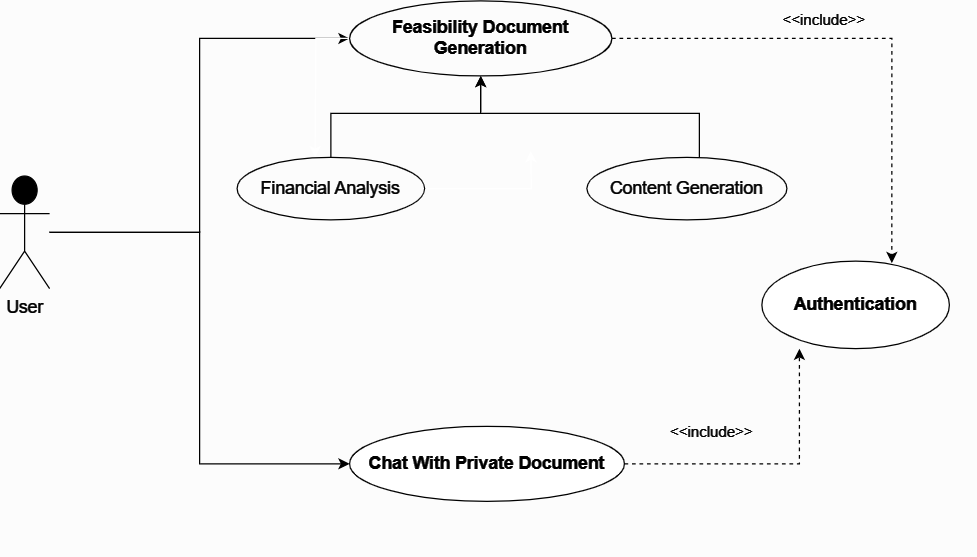
\includegraphics[width=1 \linewidth]{assets/diag.png}
    \caption{Use case diagram}
    \label{fig:usecase}
\end{figure}

\section{Technical specification}
\subsection{Non-functionnal needs}
The system must address non-functional requirements that are not essential to its operation but crucial for ensuring service quality and smooth system functioning. Non-functional requirements are internal system requirements essential for achieving our objective. To achieve this, the following requirements must be met:
\begin{itemize}
    \item \textbf{ergonomics}: Our product must feature an easy-to-use, user-friendly interface that optimizes interaction between humans and the system, even for inexperienced users. Users should be able to navigate the system effortlessly and access its functionalities without requiring any technical training.
    \item  \textbf{performance}:  Its crucial that our system must be optimized for efficiency to ensure fast response times and efficient handling of requests by reducing latency qnd improving resource utilization
    \item \textbf{Reliability}: The system should be highly reliable, with minimal downtime and disruption.The AI assistance should possess contextual awareness of the PPP project and deliver precise results consistently. 
    \item \textbf{Scalability}: The system should be scalable, capable of efficiently adapting to future demands and user growth without compromising performance.
    \item \textbf{Security }: Our system prioritizes robust security measures to safeguard sensitive data, prevent unauthorized access, and maintain compliance with industry regulations.  
\end{itemize}
\subsection{Hardware environment}
In total, our hardware environment consists of two laptops, as shown in the following \textbf{Table \ref{tab:HWE}}.

\begin{table}[h!]
\begin{center}
\caption{Hardware environment}
\label{tab:HWE}
\begin{tabular}{{|c|p{5cm}|p{5cm}|}}
\hline
\rowcolor[gray]{0.8} \bfseries{Specification} & \bfseries{HP Pavilion Gaming Laptop} & \textbf{Dell laptop} \\ 
\textbf{Operating System}       & Microsoft Windows 11 Famille Unilingue & Not specified \\
\hline
\textbf{CPU}     & Intel Core i5-10300H (2.50 GHz, 4 cores, 8 logical processors) & Intel Core \\ 
\hline
\textbf{RAM}     & 32 GB total physical memory + 36.5 GB virtual memory & Not specified \\ 
\hline
\textbf{GPU}     & NVIDIA GeForce GTX 1650 Ti & MX330 \\ 
\hline
\textbf{Storage} & 500GB & 500GB \\ 
\hline 
\end{tabular}
\end{center}
\end{table}

\subsection{Software environment}
Our adopted software are Python, LangChain, Ollama, PostgreSQL, Docker, Streamlit and LangFuse, as shown in the following table 2.2.


\begin{longtable}{|p{4cm}|p{10cm}|}
    \caption{Software environment}\label{tab6} \\
    \hline
    \rowcolor[gray]{0.8} \textbf{Software} & \textbf{Description} \\
    \hline 
    \endfirsthead

    \hline
    \rowcolor[gray]{0.8} \textbf{Software} & \textbf{Description} \\
    \endhead

    \hline 
    \multicolumn{2}{|r|}{\footnotesize Continued on next page} \\
    \hline
    \endfoot

    \hline
    \endlastfoot

    \raisebox{-1.55\height}{
\includegraphics[scale=0.2]{assets/python.jpg}} & 
    Python is a high-level programming language that is widely known for being beginner-friendly with an active community contributing to open-source projects. \\
    \hline
    \raisebox{-1.15\height}{
\includegraphics[scale=0.35]{assets/postgres.png}} & 
    PostgreSQL is an open-source relational database known for robustness and versatility. \\
    \hline
    \raisebox{-0.7\height}{
\includegraphics[scale=0.2]{assets/ollama.png}} & 
    Ollama allows you to run open-source large language models locally. \\
    \hline
    \raisebox{-1.5\height}{
\includegraphics[scale=0.2]{assets/langfuse.png}} & 
    LangFuse is an open-source platform designed for engineering with Large Language Models (LLMs). \\
    \hline
    \raisebox{-1.25\height}{
\includegraphics[scale=0.05]{assets/streamlit.png}} & 
    Streamlit simplifies data science app creation by focusing on Python skills instead of web development. \\
    \hline
    \raisebox{-0.9\height}{
\includegraphics[scale=0.03]{assets/Docker-Logo.png}} & 
    Docker is a platform as a service product that uses OS-level virtualization to deliver software in containers. \\
    \hline
\end{longtable}

    





\section{Conclusion}
In summary, we've addressed both functional and non-functional needs, ensuring user satisfaction and system performance. Then we have discussed the Hardware and software environment considerations in order to satisfy the non-functional requirements. In the next chapter, we will delve into exploring the landscape of artificial intelligence.




